% ------------------------------------------------------------------------------
% TYPO3 Version 10 LTS - What's New (English Version)
%
% @author	Michael Schams <schams.net>
% @license	Creative Commons BY-NC-SA 3.0
% @link		https://typo3.org/help/documentation/whats-new/
% @language	English
% ------------------------------------------------------------------------------

\section{Backend User Interface}
\begin{frame}[fragile]
	\frametitle{Backend User Interface}

	\begin{center}\huge{\color{typo3darkgrey}\textbf{Backend User Interface}}\end{center}
	\begin{center}\large{\textit{The TYPO3 administration interface is now better than ever}}\end{center}

\end{frame}

% ------------------------------------------------------------------------------
% ...

\begin{frame}[fragile]
	\frametitle{Backend User Interface}
	\framesubtitle{Backend UI Adjustments}

	Slightly altered UI of the backend modules column.

	\begin{figure}
		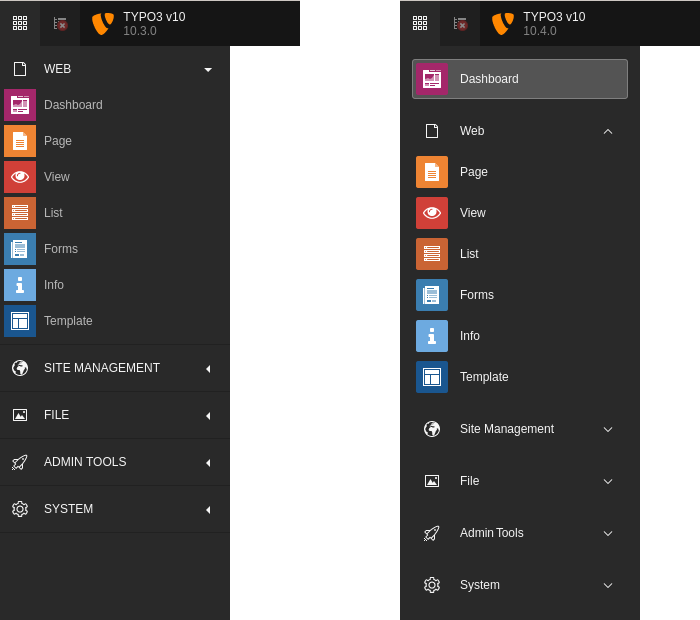
\includegraphics[width=0.5\linewidth]{BackendUserInterface/typo3-backend-ui.png}
	\end{figure}

\end{frame}

% ------------------------------------------------------------------------------
% Feature | 56213 | Allow sorting file list by file meta data title

\begin{frame}[fragile]
	\frametitle{Backend User Interface}
	\framesubtitle{Filelist Sorting}

	Files can now be sorted by their meta data title in the "File Links" content element.

	\begin{figure}
		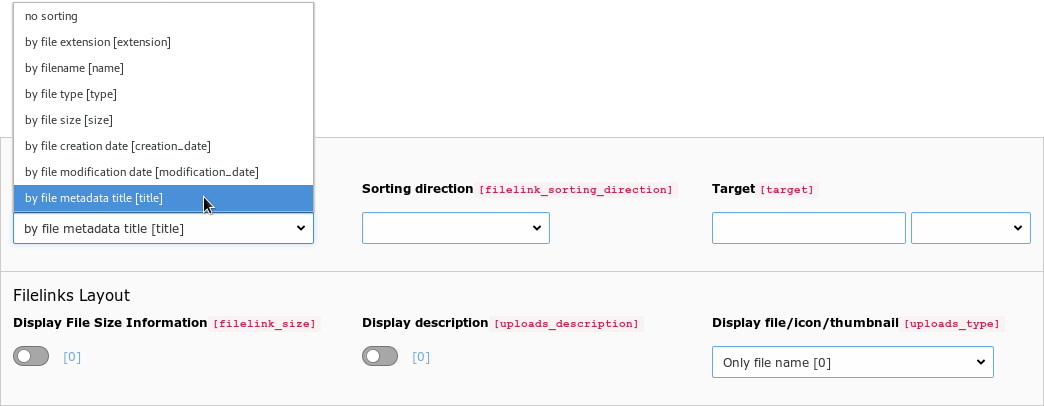
\includegraphics[width=0.90\linewidth]{BackendUserInterface/56213-FilelistSorting.png}
	\end{figure}

\end{frame}

% ------------------------------------------------------------------------------
% Feature | 85569 | Show scheduler information in the system information toolbar

\begin{frame}[fragile]
	\frametitle{Backend User Interface}
	\framesubtitle{System Information Toolbar}

	The system information toolbar now shows information about the TYPO3 scheduler.

	\begin{figure}
		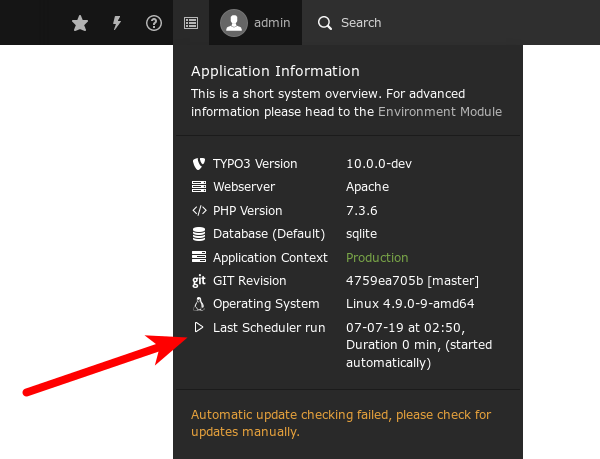
\includegraphics[width=0.50\linewidth]{BackendUserInterface/85569-SchedulerInfoInStatusBar.png}
	\end{figure}

\end{frame}

% ------------------------------------------------------------------------------
% Feature | 86629 | Implement LinkHandler for telephone numbers

\begin{frame}[fragile]
	\frametitle{Backend User Interface}
	\framesubtitle{Link Handler}

	A new link handler has been added that lets backend users set links to phone
    numbers using the \texttt{tel:} protocol.

	\begin{figure}
		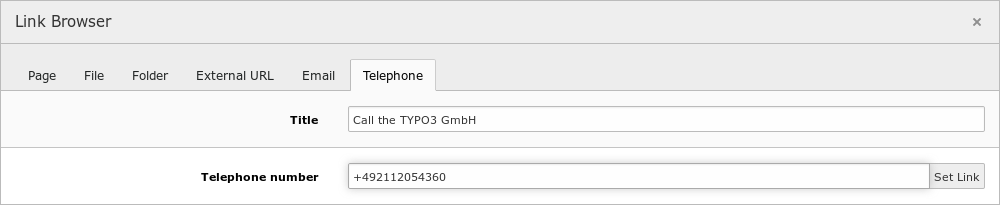
\includegraphics[width=0.90\linewidth]{BackendUserInterface/86629-TelephoneNumberLinkHandler.png}
	\end{figure}

	\begin{figure}
		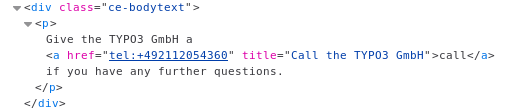
\includegraphics[width=0.60\linewidth]{BackendUserInterface/86629-TelephoneNumberLinkHandler2.png}
	\end{figure}

\end{frame}

% ------------------------------------------------------------------------------
% Feature | 87433 | Add changefreq and priority

\begin{frame}[fragile]
	\frametitle{Backend User Interface}
	\framesubtitle{\texttt{EXT:seo}: Backend View}

	The SEO system extension now supports change frequencies and priorities for the Sitemap.
	Page properties (tab "SEO") feature two new fields.

	\begin{figure}
		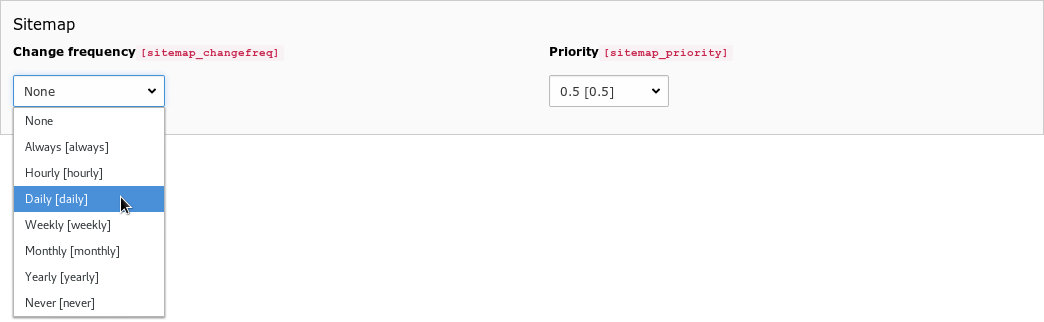
\includegraphics[width=0.90\linewidth]{BackendUserInterface/87433-SeoAddChangefreqAndPriority.png}
	\end{figure}

\end{frame}

% ------------------------------------------------------------------------------
% Feature | 87433 | Add changefreq and priority

\begin{frame}[fragile]
	\frametitle{Backend User Interface}
	\framesubtitle{\texttt{EXT:seo}: Configuration Options for Integrators}

	% decrease font size for code listing
	\lstset{basicstyle=\tiny\ttfamily}

	These settings can also be defined in TypoScript, mapped to fields in the database.

	\begin{lstlisting}
plugin.tx_seo {
  config {
    xmlSitemap {
      sitemaps {
        <unique key> {
          provider = TYPO3\CMS\Seo\XmlSitemap\RecordsXmlSitemapDataProvider
          config {
            ...
            changeFreqField = news_changefreq
            priorityField = news_priority
            ...
          }
        }
      }
    }
  }
}
	\end{lstlisting}

\end{frame}

% ------------------------------------------------------------------------------
% Feature | 83128 | Content Element Filter

\begin{frame}[fragile]
	\frametitle{Backend User Interface}
	\framesubtitle{New Content Element Search}

	Backend users can now search for content element types in the "New Content Element" wizard:

	\begin{figure}
		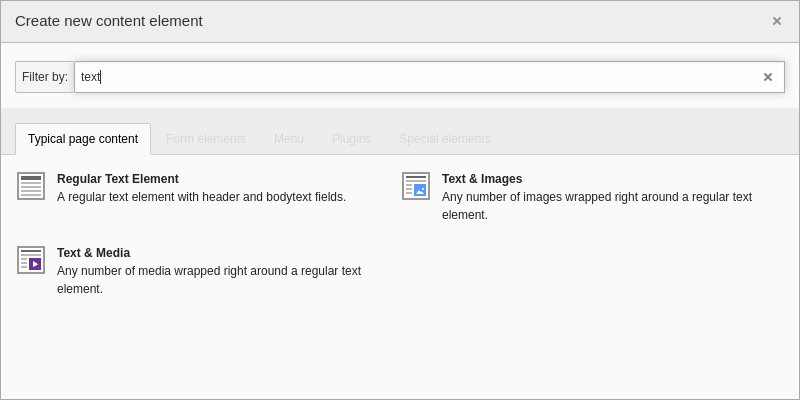
\includegraphics[width=0.6\linewidth]{BackendUserInterface/83128-ContentElementFilter.png}
	\end{figure}

\end{frame}

% ------------------------------------------------------------------------------
% Feature | 85918 | Hide in menu / Show in menu entry for pages in context menu

\begin{frame}[fragile]
	\frametitle{Backend User Interface}
	\framesubtitle{Hide/Show in Menu}

	A new entry was added to the context menu to show/hide pages in the menu.

	\begin{figure}
		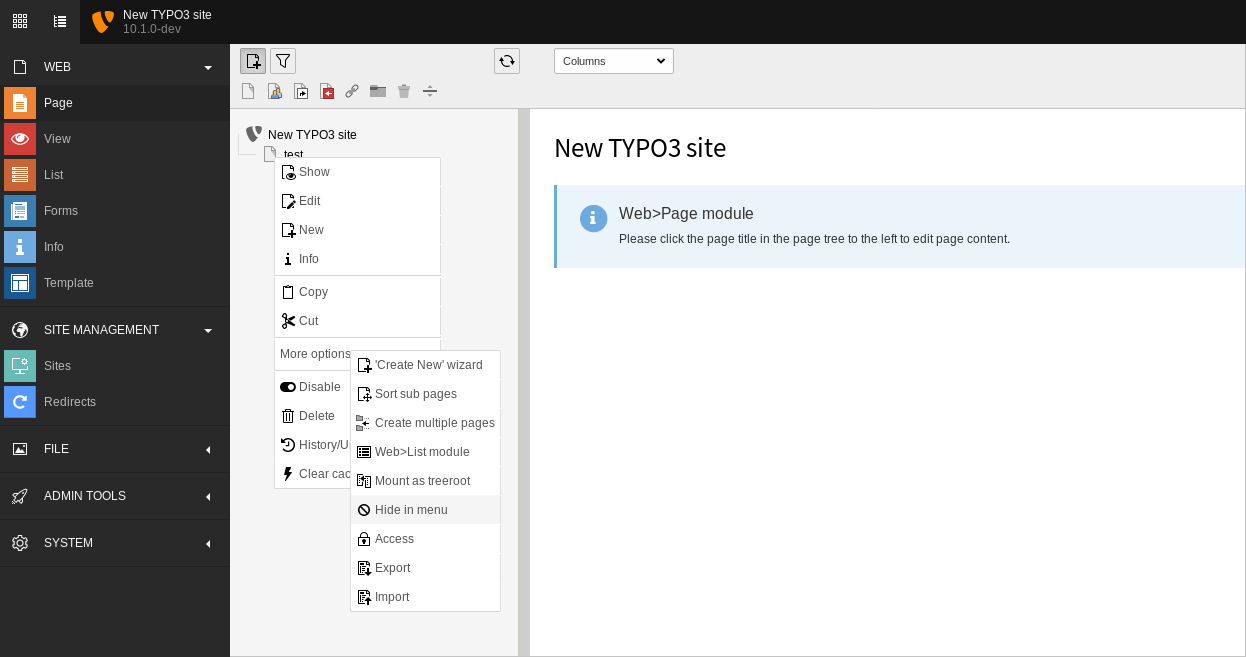
\includegraphics[width=0.80\linewidth]{BackendUserInterface/85918-HideShowInMenu-InContextMenu.png}
	\end{figure}

\end{frame}

% ------------------------------------------------------------------------------
% Feature | 89458 | Show link to online docs in extension manager

\begin{frame}[fragile]
	\frametitle{Backend User Interface}
	\framesubtitle{Extension Manager}

	The Extension Manager now shows links to extension documentation.

	\begin{figure}
		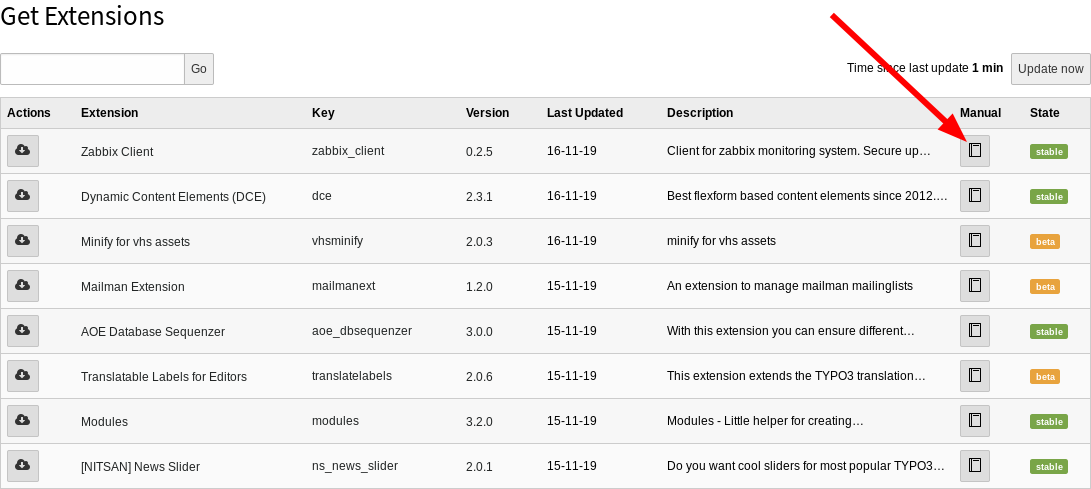
\includegraphics[width=0.90\linewidth]{BackendUserInterface/89458-ShowLinkToOnlineDocsInExtensionManager.png}
	\end{figure}

\end{frame}

% ------------------------------------------------------------------------------
% Feature | 89894 | Separate system extensions from 3rd-party extensions visually

\begin{frame}[fragile]
	\frametitle{Backend User Interface}
	\framesubtitle{Extension Manager}

	System and 3rd-party extensions can now be listed separately in the Extension Manager.

	\begin{figure}
		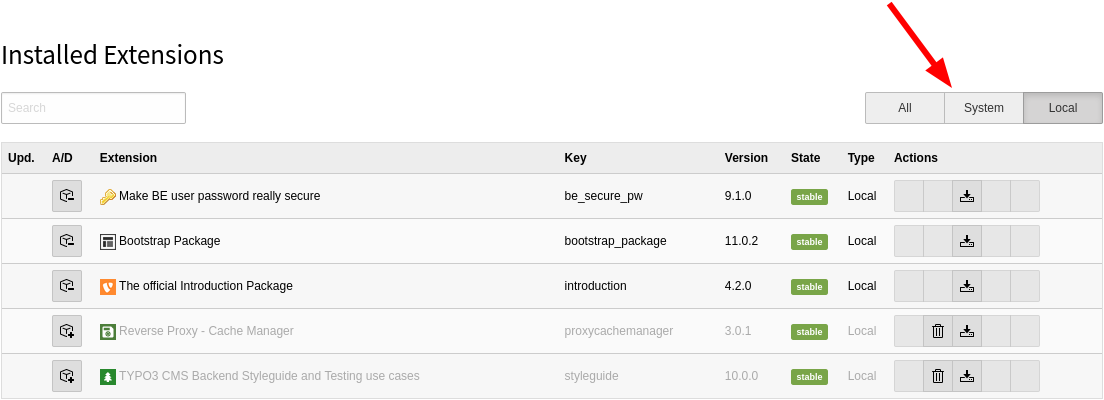
\includegraphics[width=0.9\linewidth]{BackendUserInterface/89894-SeparateSystemExtensionsFrom3rdPartyExtensionsVisually.png}
	\end{figure}

\end{frame}

% ------------------------------------------------------------------------------
% Feature | 86818 | Reintroduce keyboard accessible version of the pagetree

\begin{frame}[fragile]
	\frametitle{Backend User Interface}
	\framesubtitle{Pagetree Accessibility}

	Backend users can now use their keyboard to navigate through the pagetree.
	For example the arrow keys, "home", "end", "enter", "space", etc.
	\newline
	This is in accordance to the best practices as described in
	\href{https://www.w3.org/TR/wai-aria-practices-1.1/#keyboard-interaction-22}{WAI-ARIA Authoring Practices 1.1}
	by the W3C.

	\begin{figure}
		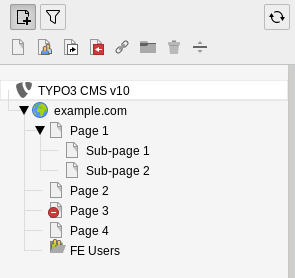
\includegraphics[width=0.30\linewidth]{BackendUserInterface/86818-PagetreeAccessibility.png}
	\end{figure}

\end{frame}

% ------------------------------------------------------------------------------
% Feature | 90298 | Improve user info in BE User module

\begin{frame}[fragile]
	\frametitle{Backend User Interface}
	\framesubtitle{Backend User Module}

	\begin{itemize}
		\item A new detail view of backend user records shows all relevant data.
		\item Additional fields have been added to the function to compare users.
		\item This function also takes subgroups into account now.
		\item The user interface of the module will be adjusted and optimized further.
		\item These changes make it easier for integrators/administrators to check
			and compare user permissions without switching to the user.
	\end{itemize}

\end{frame}

% ------------------------------------------------------------------------------
% Feature | 90826 | Compare backend usergroups

\begin{frame}[fragile]
	\frametitle{Backend User Interface}
	\framesubtitle{Backend User Module}

	\begin{itemize}
		\item Integrators are now able to compare individual backend usergroups.
	\end{itemize}

	\begin{figure}
		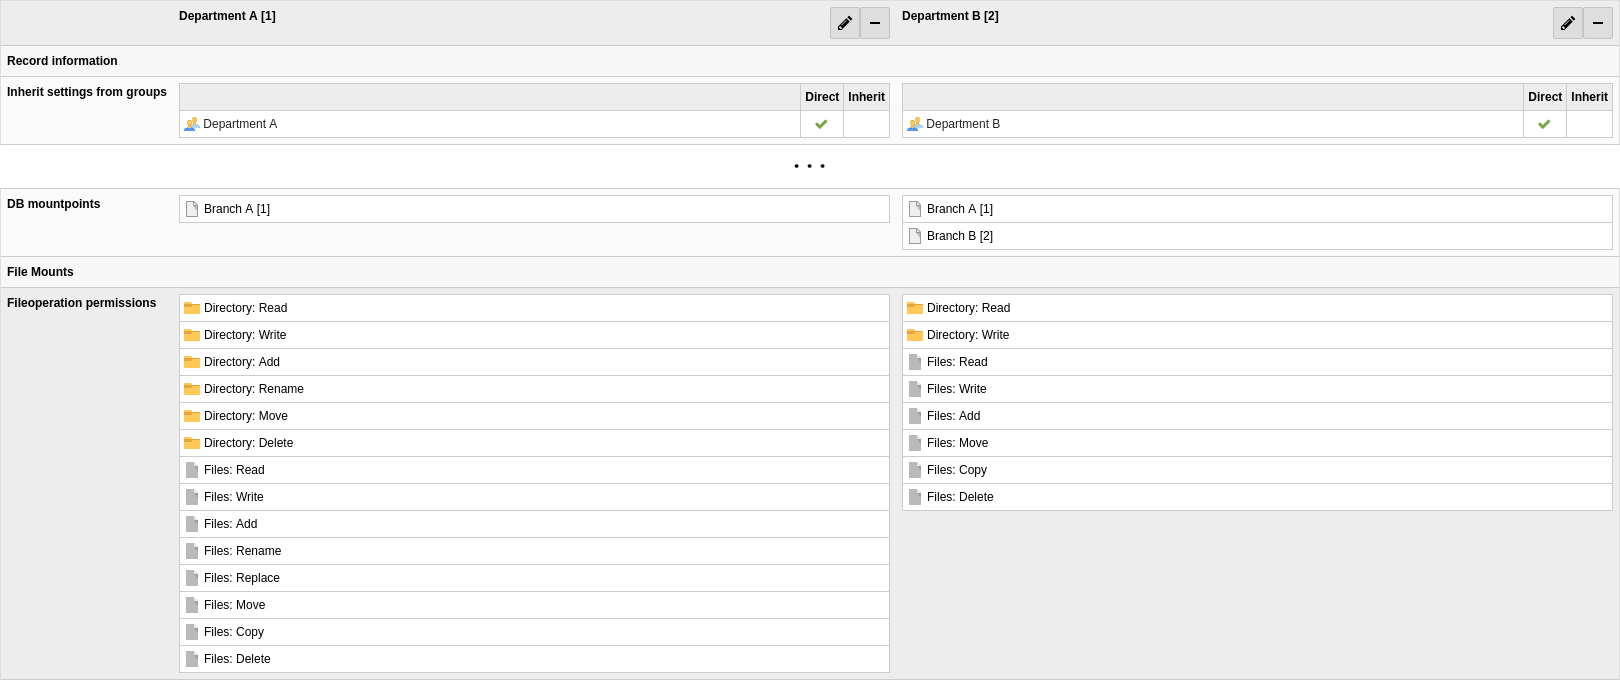
\includegraphics[width=0.9\linewidth]{BackendUserInterface/90826-CompareBackendUsergroups.png}
	\end{figure}

\end{frame}

% ------------------------------------------------------------------------------
% Feature | 90136 | Show application context in the Environment module

\begin{frame}[fragile]
	\frametitle{Backend User Interface}
	\framesubtitle{Environment Overview}

	The current application context is now shown in the Environment module:\newline
	\textbf{ADMIN TOOLS} $\rightarrow$ \textbf{Environment} $\rightarrow$ \textbf{Environment Overview}.

	\begin{figure}
		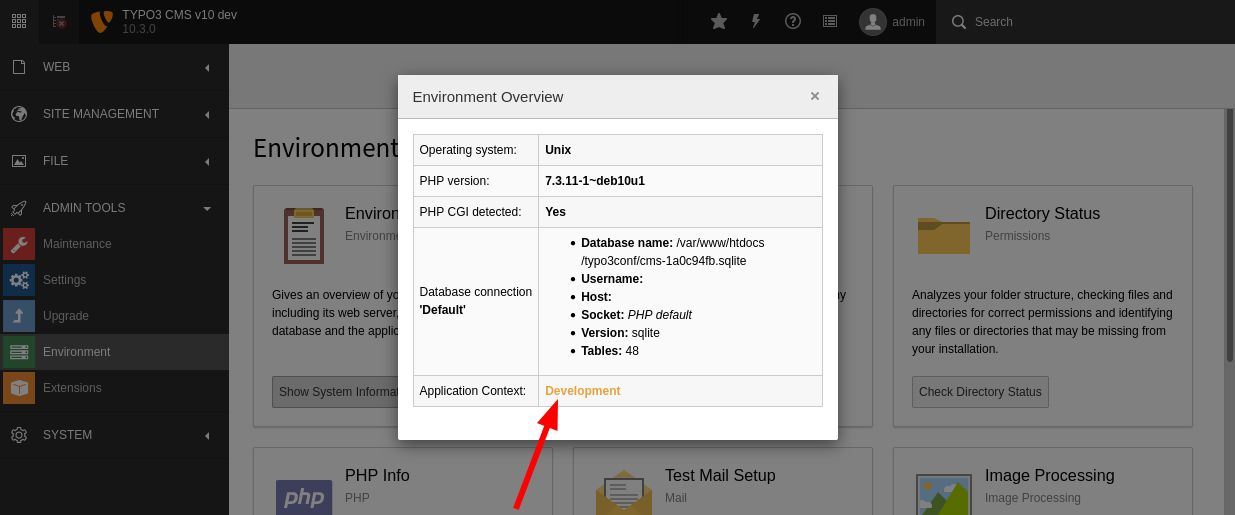
\includegraphics[width=0.9\linewidth]{BackendUserInterface/90136-ShowApplicationContextInTheEnvironmentModule.png}
	\end{figure}

\end{frame}

% ------------------------------------------------------------------------------
% Task | 89844 | Improve visual appearance of feature toggles

\begin{frame}[fragile]
	\frametitle{Backend User Interface}
	\framesubtitle{Feature Toggles}

	The visual appearance of feature toggles has been improved:
	\newline\newline
	\smaller\textbf{TYPO3 v9 LTS}\tabto{6cm}\textbf{TYPO3 v10 LTS}\normalsize

	\begin{figure}
		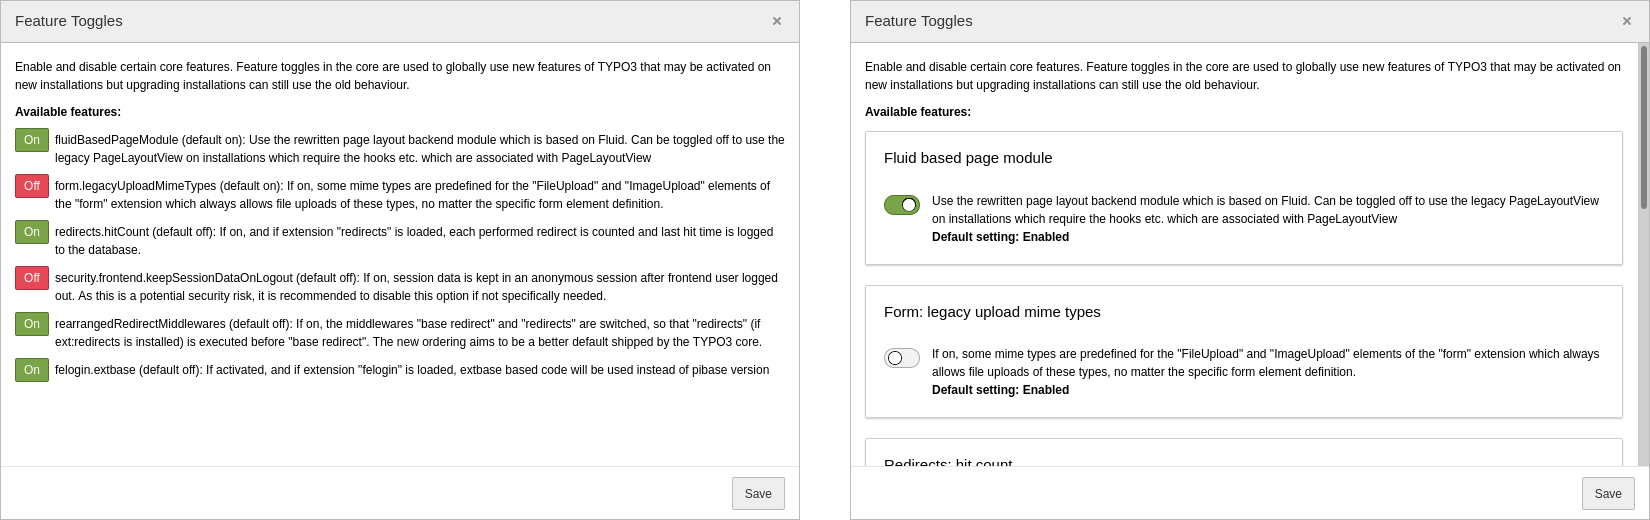
\includegraphics[width=1\linewidth]{InDepthChanges/89844-ImproveVisualAppearanceOfFeatureToggles.png}
	\end{figure}

\end{frame}

% ------------------------------------------------------------------------------
% Feature | 90425 | Add seo fields to info module

\begin{frame}[fragile]
	\frametitle{Backend User Interface}
	\framesubtitle{Info Module}

	\begin{itemize}
		\item SEO and Social Media details have been added to the Info module:\newline
			\textbf{WEB} $\rightarrow$ \textbf{Info} $\rightarrow$ \textbf{Pagetree Overview}.
	\end{itemize}

	\begin{figure}
		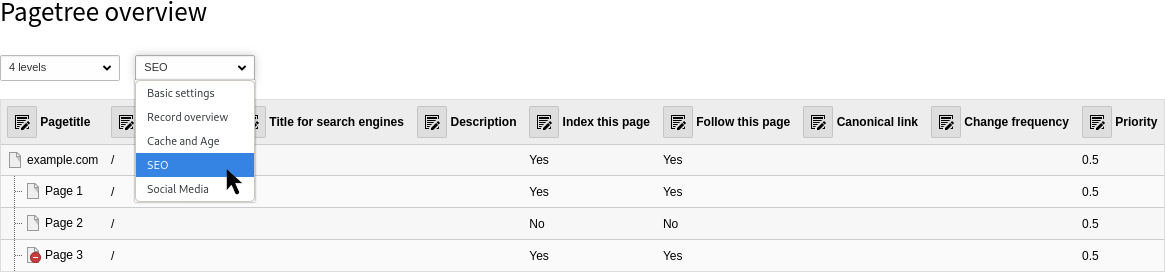
\includegraphics[width=0.85\linewidth]{BackendUserInterface/90425-AddSeoFieldsToInfoModule.png}
	\end{figure}

\end{frame}

% ------------------------------------------------------------------------------
% Feature | 89513 | Provide password recovery for backend users

\begin{frame}[fragile]
	\frametitle{Backend User Interface}
	\framesubtitle{Password Reset for Backend Users}

	Backend users can now request a password recovery email to reset their access details.

	\begin{figure}
		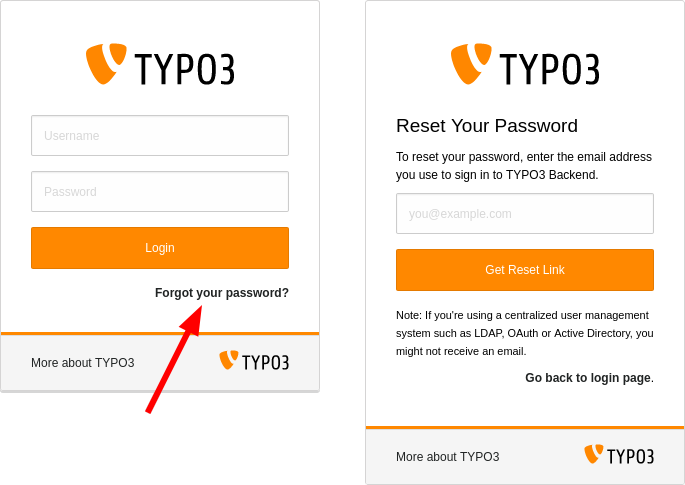
\includegraphics[width=0.55\linewidth]{BackendUserInterface/89513-ProvidePasswordRecoveryForBackendUsers.png}
	\end{figure}

\end{frame}

% ------------------------------------------------------------------------------
% Feature | 89513 | Provide password recovery for backend users

\begin{frame}[fragile]
	\frametitle{Backend User Interface}
	\framesubtitle{Password Reset for Backend Users}

	\begin{itemize}

		\item Password resets for backend users are only valid for 4 hours.\newline
			This time limit is not configurable.
		\item To strengthen security, the function can be disabled for admin users or for all users.
		\item If users share one email address, an alternative email text is used.
		\item TCA field \texttt{be\_users.email} must not be set to \texttt{eval=email}.

		\item The function only works for users, who:
			\begin{itemize}
				\item have an email address set,
				\item have a password set, and
				\item are not disabled/deleted.
			\end{itemize}

	\end{itemize}

\end{frame}

% ------------------------------------------------------------------------------
% Feature | 89513 | Provide password recovery for backend users

\begin{frame}[fragile]
	\frametitle{Backend User Interface}
	\framesubtitle{Password Reset for Backend Users}

	\begin{itemize}
		\item Password recovery emails can also be triggered on the command line.
	\end{itemize}

	\begin{figure}
		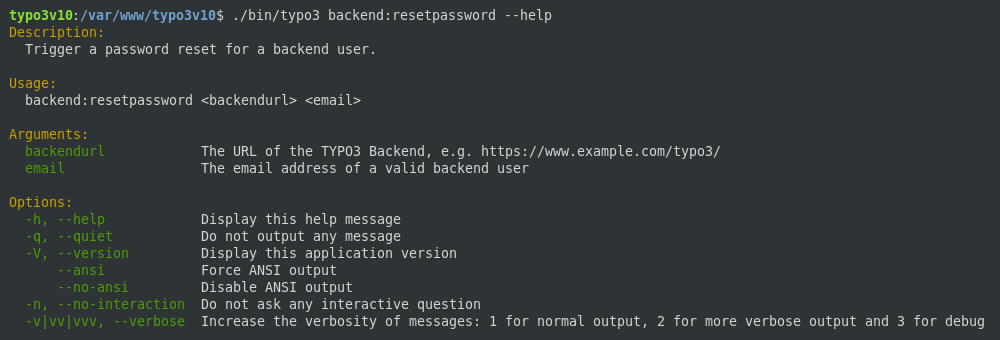
\includegraphics[width=0.9\linewidth]{BackendUserInterface/89513-BackendPasswordResetCommandLine.png}
	\end{figure}

\end{frame}

% ------------------------------------------------------------------------------
% Feature | 89115 | Auto slug update and redirect creation on slug change

\begin{frame}[fragile]
	\frametitle{Backend User Interface}
	\framesubtitle{Slug Updates and Redirects}

	\begin{itemize}
		\item When backend users change the URL path of a page (the so-called "slug"),
			the old URL becomes unavailable.
		\item This possibly results in a "page not found" error for this page,
			including the URLs of all sub-pages.
	\end{itemize}

	\begin{figure}
		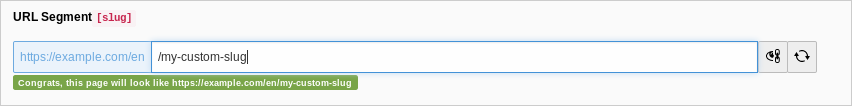
\includegraphics[width=0.80\linewidth]{BackendUserInterface/89115b-AutoSlugUpdateAndRedirectCreationOnSlugChange.png}
	\end{figure}

	\begin{itemize}
		\item Two actions prevent this from happening now:

			\begin{itemize}
				\item slugs for all sub-pages are automatically updated
				\item redirects from the old to the new URLs are created
			\end{itemize}

	\end{itemize}

\end{frame}

% ------------------------------------------------------------------------------
% Feature | 89115 | Auto slug update and redirect creation on slug change

\begin{frame}[fragile]
	\frametitle{Backend User Interface}
	\framesubtitle{Slug Updates and Redirects}

	\begin{itemize}
		\item Backend users are informed about these actions and they can
			easily roll back the changes with a click of a button if required:
	\end{itemize}

	\begin{figure}
		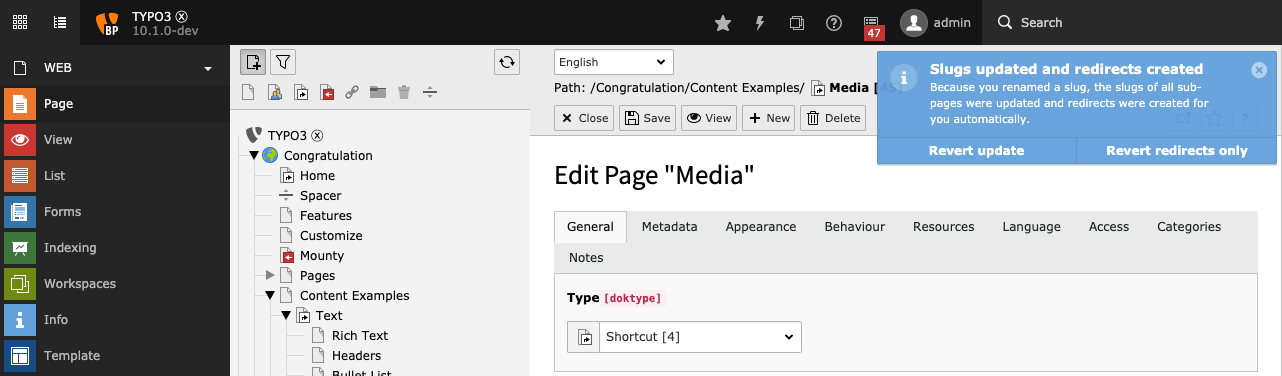
\includegraphics[width=0.80\linewidth]{BackendUserInterface/89115c-AutoSlugUpdateAndRedirectCreationOnSlugChange.png}
	\end{figure}

\end{frame}

% ------------------------------------------------------------------------------
